\red{En esta sección se presenta una descripción detallada de todo lo relacionado con el desarrollo de del proyecto, se abarcan los temas relacionados con la Ingeniería de Software, así como los procesos seguidos y tecnologías utilizadas. Permite conocer los procesos seguidos desde la planificación planteada inicialmente hasta la finalización del proyecto, incluyendo las desviaciones ocurridas}

\section{Planificación y seguimiento} \label{sec:plan}
% deberase incluír un diagrama de Gantt que amose tanto
% a planificación do traballo, coa súa distribución de fases e tarefas, e a súa comparación cos
% datos reais obtidos tras o desenvolvemento do traballo.
    
    Como se expone en el apartado \ref{sec:sol}, la metodología de desarrollo elegida para este proyecto es \textit{SCRUM}.  En este apartado se explica cómo se llevan a cabo todas sus fases, las historias de usuario y tareas incluidas en cada una de ellas, y las desviaciones ocurridas.
    
    \subsection{Historias de usuario}
    
        A continuación se presentan las historias de usuario planteadas inicialmente:
    
        \begin{tabular}{ll}
            \textbf{Como}   & \red{desarrollador}                                                   \\
            
            \textbf{Quiero} & que el sistema sea modular                                            \\
            
            \textbf{Para}   & incorporar nuevas funcionalidades sin modificar el sistema            \\
        \end{tabular}
    
        \begin{tabular}{ll}
            \textbf{Como}   & administrador                                                         \\
            
            \textbf{Quiero} & ejecutar la aplicación como un servicio                               \\
            
            \textbf{Para}   & que se mantenga permanentemente en ejecución                          \\
        \end{tabular}
        
        \begin{tabular}{ll}
            \textbf{Como}   & administrador                                                         \\
            
            \textbf{Quiero} & ejecutar la aplicación desde la consola de comandos                   \\
            
            \textbf{Para}   & realizar ejecuciones manuales                                         \\
        \end{tabular}
        
        \begin{tabular}{ll}
            \textbf{Como}   & administrador                                                         \\
            
            \textbf{Quiero} & especificar la configuración en un archivo                            \\
            
            \textbf{Para}   & desplegar el sistema fácilmente en varios servidores                  \\
        \end{tabular}
        
        \begin{tabular}{ll}
            \textbf{Como}   & administrador                                                         \\
            
            \textbf{Quiero} & capturar eventos del sistema en tiempo real                           \\
            
            \textbf{Para}   & detectar errores en el servidor lo antes posible                      \\
        \end{tabular}
        
        \begin{tabular}{ll}
            \textbf{Como}   & administrador                                                         \\
            
            \textbf{Quiero} & que la aplicación se actualice automáticamente                        \\
            
            \textbf{Para}   & tener siempre la aplicación actualizada en todos los servidores       \\
        \end{tabular}
        
        \begin{tabular}{ll}
            \textbf{Como}   & administrador                                                         \\
            
            \textbf{Quiero} & obtener información de las actualizaciones del Sistema Operativo      \\
            
            \textbf{Para}   & controlar los servidores desactualizados                              \\
        \end{tabular}
        
        \begin{tabular}{ll}
            \textbf{Como}   & administrador                                                         \\
            
            \textbf{Quiero} & tener un sistema de latidos                                           \\
            
            \textbf{Para}   & saber cuando un servidor ha fallado                                   \\
        \end{tabular}
        
        \begin{tabular}{ll}
            \textbf{Como}   & administrador                                                         \\
            
            \textbf{Quiero} & que la información sea mostrada en consola                            \\
            
            \textbf{Para}   & depurar error con comprobaciones manuales                             \\
        \end{tabular}
        
        \begin{tabular}{ll}
            \textbf{Como}   & administrador                                                         \\
            
            \textbf{Quiero} & que la información se envíe a un servidor RabbitMQ                    \\
            
            \textbf{Para}   & poder consumirla con otros sistemas                                   \\
        \end{tabular}
        
    \subsection{Planificación inicial}
        Como se muestra en la tabla \ref{tab:fases-planif}, el desarrollo del sistema se llevará a cabo durante nueve fases, entre las cuales se incluyen cinco \textit{sprints} de implementación y la elaboración de la documentación, que incluye la fase de cierre, fundamental en \textit{SCRUM}
            
        \begin{table}[h!]             
            \centering                  
                \resizebox{\textwidth}{!}{   
                    \begin{tabular}{|l|c|c|}
                        \hline
                        \multirow{2}{*}{\textbf{Fase}}      & \multicolumn{2}{|c|}{\textbf{Estimación temporal}}    \\
                        \cline{2-3}
                                                            &   Días                &   Horas                       \\
                        \hline
                        Spike                               &   4                   &   12                          \\
                        Pruebas con diferentes lenguajes    &   4                   &   12                          \\
                        Boceto                              &   2                   &   6                           \\
                        Sprint 1                            &   15                  &   45                          \\
                        Sprint 2                            &   15                  &   45                          \\
                        Sprint 3                            &   15                  &   45                          \\
                        Sprint 4                            &   15                  &   45                          \\
                        Sprint 5                            &   10                  &   30                          \\
                        \hline
                        \hline
                        Documentación                       &   80                  &   240                         \\
                        \hline                  
                        \hline                  
                        \textbf{Total}                      &   \textbf{80}         &   \textbf{240}                \\
                        \hline
                    \end{tabular}
                }
            \caption{Planificación de las fases}
            \label{tab:fases-planif}
        \end{table}
        
        En las imágenes \ref{fig:gantt-initial-tasks} y \ref{fig:gantt-initial-diagram} se puede apreciar la planificación en el tiempo de las nueve fases antes mencionadas.
        
        \begin{figure}[h!]
        \centering
            \frame{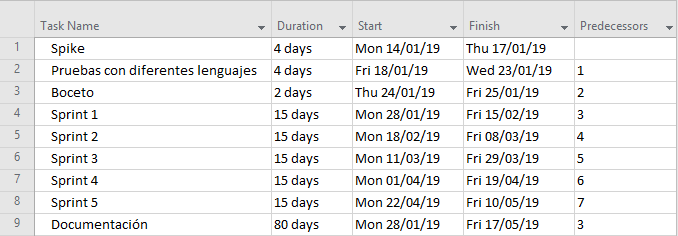
\includegraphics[scale=0.7]{planificacion-inicial-tareas.png}}
            \caption{Planificación de las fases del proyecto}
            \label{fig:gantt-initial-tasks}
        \end{figure}
        
        \begin{figure}[h!]
        \centering
            \frame{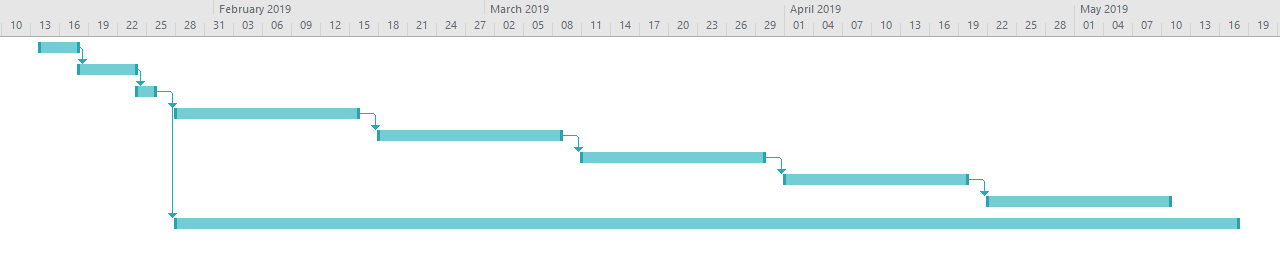
\includegraphics[scale=0.44]{planificacion-inicial-diagrama.png}}
            \caption{Diagrama de Gantt de la planificación inicial}
            \label{fig:gantt-initial-diagram}
        \end{figure}
        
    \subsection{Seguimiento del proyecto}
        
        Las imágenes \ref{fig:gantt-followup-tasks} y \ref{fig:gantt-followup-diagram} muestran la planificación detallada de las tareas del proyecto. Es importante destacar que debido a actividades no relacionadas con la aplicación, o actividades que aunque sean relacionadas con la aplicación, no son incluidas en este proyecto, el proceso de desarrollo se ha visto afectado en ciertos momentos. \red{poner cómo lo ha afectado?}
        
        \begin{figure}[h!]
        \centering
            \frame{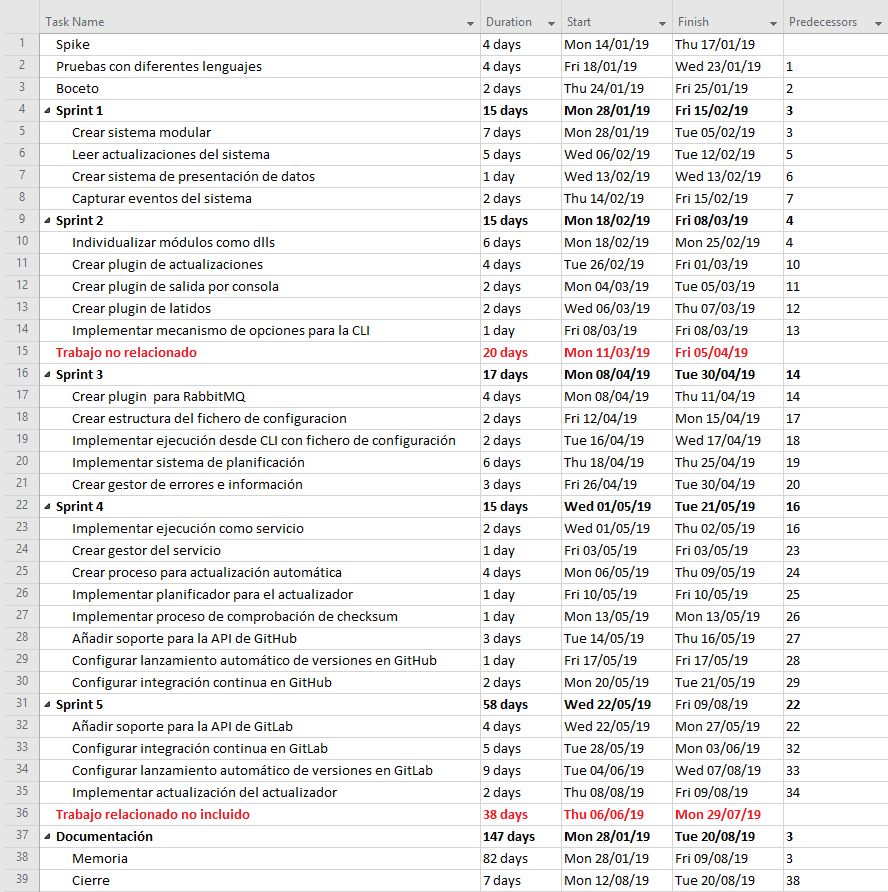
\includegraphics[scale=0.6]{seguimiento-tareas.png}}
            \caption{Planificación de las tareas del proyecto}
            \label{fig:gantt-followup-tasks}
        \end{figure}
    
        \begin{figure}[h!]
        \centering
            \frame{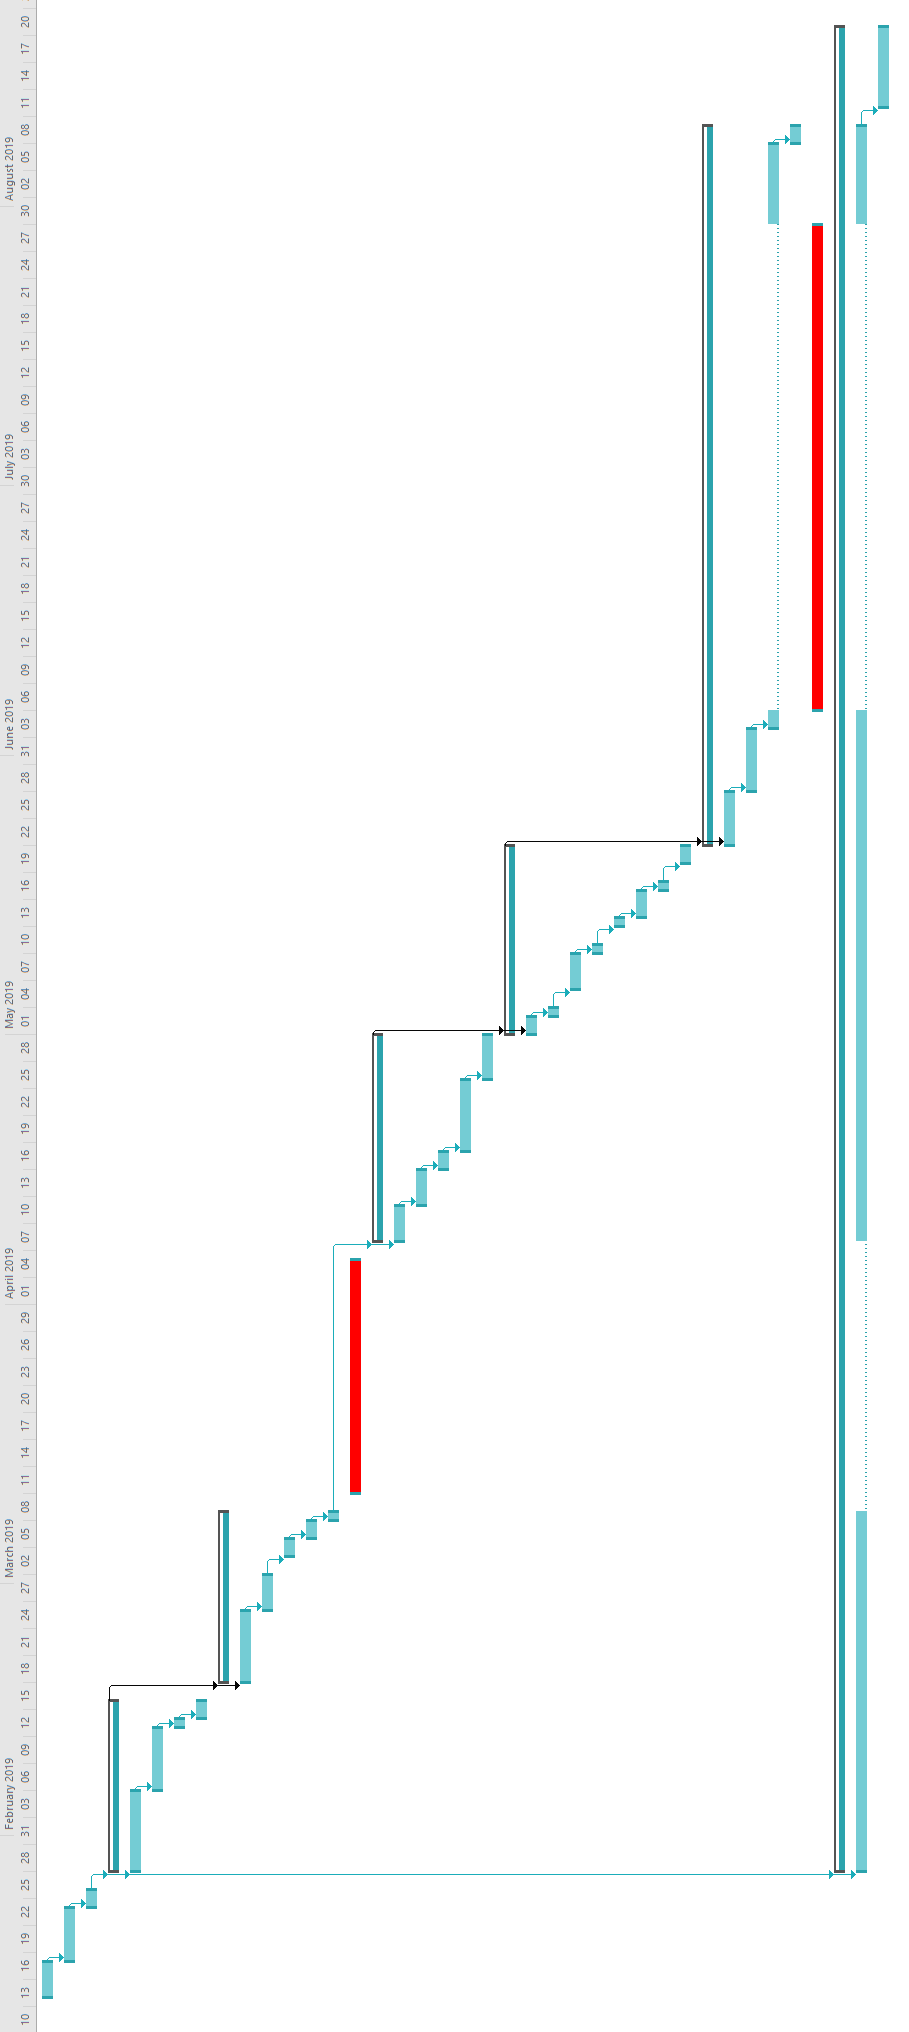
\includegraphics[scale=0.44]{seguimiento-diagrama.png}}
            \caption{Diagrama de Gantt de la planificación de tareas}
            \label{fig:gantt-followup-diagram}
        \end{figure}